% generated by scripts/pkl_to_latex.py
% source PKL : uscan_v1_L8_Ne8_t0p1_mode-uniform_nmin2_solver-gcg_full_es_restarts10_iter300_kmax5_tol1em09_U0.1to5_N21-8081b758e7cc.pkl
% scan type  : uscan
% state      : ex_singlet
% quantity   : vn-entropy
% requires   : \usepackage{pgfplots} \pgfplotsset{compat=1.18}
% colours match the matplotlib PDF (tab10 cycle)
\definecolor{gmeC0}{HTML}{1F77B4}
\definecolor{gmeC1}{HTML}{FF7F0E}
\definecolor{gmeC2}{HTML}{2CA02C}
\definecolor{gmeC3}{HTML}{D62728}
\definecolor{gmeC4}{HTML}{9467BD}
\definecolor{gmeC5}{HTML}{8C564B}
\definecolor{gmeC6}{HTML}{E377C2}
\definecolor{gmeC7}{HTML}{17BECF}

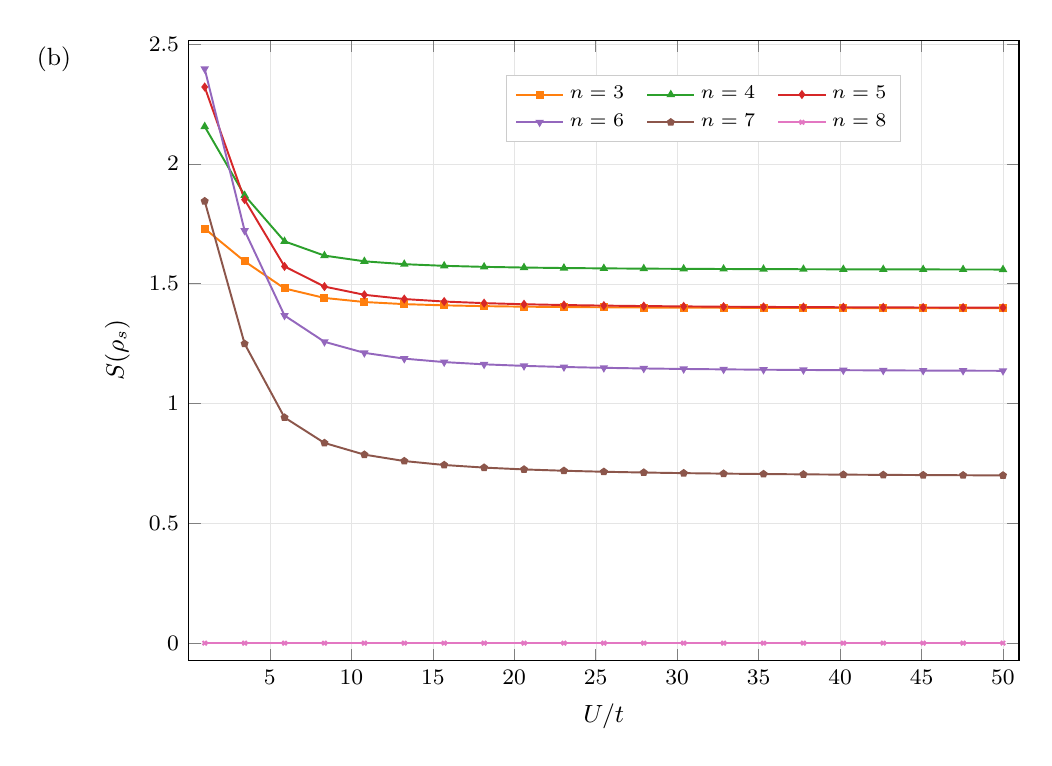
\begin{tikzpicture}
  \begin{axis}[
    width=\columnwidth,
    height=0.78\columnwidth,
    xlabel={$U/t$},
    ylabel={$S(\rho_s)$},
    grid=both,
    grid style={line width=.1pt, draw=gray!20},
    tick label style={font=\footnotesize\rmfamily, /pgf/number format/fixed},
    label style={font=\small\rmfamily},
    scaled ticks=false,
    legend style={font=\scriptsize\rmfamily, draw=gray!40, at={(0.5,1.03)}, anchor=south, /tikz/every even column/.append style={column sep=6pt}},
    legend cell align={left},
    legend columns=3,
    ymin=-0.072,
    ymax=2.516,
    xmin=0.02,
    xmax=50.98,
    legend style={at={(0.620,0.890)}, anchor=center, fill=white},
    after end axis/.append code={\node[anchor=east, font=\small\rmfamily] at (axis description cs:-0.13,0.970) {(b)};},
  ]
    \addplot[color=gmeC1, mark=square*, mark size=1.1pt, line width=0.7pt] coordinates {
        (1,1.729755) (3.45,1.593234) (5.9,1.480039) (8.35,1.440402)
        (10.8,1.42341) (13.25,1.414592) (15.7,1.409441) (18.15,1.406177)
        (20.6,1.403983) (23.05,1.402439) (25.5,1.401311) (27.95,1.400464)
        (30.4,1.39981) (32.85,1.399297) (35.3,1.398885) (37.75,1.398551)
        (40.2,1.398275) (42.65,1.398045) (45.1,1.397852) (47.55,1.397687)
        (50,1.397546)
    };
    \addlegendentry{$n=3$}
    \addplot[color=gmeC2, mark=triangle*, mark size=1.1pt, line width=0.7pt] coordinates {
        (1,2.155755) (3.45,1.868452) (5.9,1.676586) (8.35,1.617114)
        (10.8,1.593238) (13.25,1.581261) (15.7,1.574396) (18.15,1.570098)
        (20.6,1.56723) (23.05,1.565223) (25.5,1.563763) (27.95,1.562668)
        (30.4,1.561826) (32.85,1.561165) (35.3,1.560637) (37.75,1.560208)
        (40.2,1.559854) (42.65,1.55956) (45.1,1.559312) (47.55,1.559102)
        (50,1.558921)
    };
    \addlegendentry{$n=4$}
    \addplot[color=gmeC3, mark=diamond*, mark size=1.1pt, line width=0.7pt] coordinates {
        (1,2.320584) (3.45,1.850505) (5.9,1.571885) (8.35,1.487816)
        (10.8,1.453501) (13.25,1.43582) (15.7,1.425398) (18.15,1.418696)
        (20.6,1.414114) (23.05,1.410833) (25.5,1.408397) (27.95,1.406537)
        (30.4,1.405081) (32.85,1.40392) (35.3,1.402978) (37.75,1.402203)
        (40.2,1.401556) (42.65,1.401011) (45.1,1.400547) (47.55,1.400149)
        (50,1.399805)
    };
    \addlegendentry{$n=5$}
    \addplot[color=gmeC4, mark=triangle*, mark size=1.1pt, mark options={rotate=180}, line width=0.7pt] coordinates {
        (1,2.396406) (3.45,1.721181) (5.9,1.367123) (8.35,1.257416)
        (10.8,1.211319) (13.25,1.187143) (15.7,1.172715) (18.15,1.163351)
        (20.6,1.156899) (23.05,1.152251) (25.5,1.148782) (27.95,1.14612)
        (30.4,1.144029) (32.85,1.142355) (35.3,1.140993) (37.75,1.139868)
        (40.2,1.138928) (42.65,1.138133) (45.1,1.137456) (47.55,1.136873)
        (50,1.136367)
    };
    \addlegendentry{$n=6$}
    \addplot[color=gmeC5, mark=pentagon*, mark size=1.1pt, line width=0.7pt] coordinates {
        (1,1.844291) (3.45,1.249203) (5.9,0.941509) (8.35,0.83526)
        (10.8,0.786596) (13.25,0.759793) (15.7,0.743318) (18.15,0.732414)
        (20.6,0.724798) (23.05,0.719255) (25.5,0.715086) (27.95,0.711867)
        (30.4,0.709325) (32.85,0.707282) (35.3,0.705613) (37.75,0.704231)
        (40.2,0.703072) (42.65,0.702091) (45.1,0.701253) (47.55,0.70053)
        (50,0.699902)
    };
    \addlegendentry{$n=7$}
    \addplot[color=gmeC6, mark=x, mark size=1.1pt, line width=0.7pt] coordinates {
        (1,0) (3.45,0) (5.9,0) (8.35,0)
        (10.8,0) (13.25,0) (15.7,0) (18.15,0)
        (20.6,0) (23.05,0) (25.5,0) (27.95,0)
        (30.4,0) (32.85,0) (35.3,0) (37.75,0)
        (40.2,0) (42.65,0) (45.1,0) (47.55,0)
        (50,0)
    };
    \addlegendentry{$n=8$}
  \end{axis}
\end{tikzpicture}
